%! TEX root = ../main.tex
\documentclass[../main]{subfiles}

% ローカル下書き用
% \documentclass{supernova_pre}
% このクラスの中に大体のパッケージは入ってるので基本何でもかけるはず
% 追加したいパッケージがあればここに記入


\begin{document}
\chapter{星座早見盤を3D化したい} % タイトル
\rightline{M1 藤澤春風} % 学年と名前(ハンドルネームでも可)


%_________________星座早見盤の描画______________________
\section{星座早見盤の描画}
「Pythonで星座早見盤を描画して、俺の夏休みの自由研究にする!」

同じく大学院1年の天文部員がそんなことを言い始めたのは、長い夏休みを半分ほど浪費してしまった9月某日のことである。最初は彼一人でコードを書いていたが、彼の書くコードはあまりにも悲惨だった。これを見かねて手助けしたのが、この「星座早見盤3D化計画(?)」の始まりである。

最初に作成したのは、日時(年月日時分秒)と場所(緯度経度)を入力すると、その日時にその場所から見える星空を描画してくれるプログラムである。よく見る星座早見盤は日時の指定しかできないが、今回はせっかくなので場所の指定もできるようにした。
過去の部誌には、優秀な先輩が残してくれた「今日の星空を計算したい$^\text{\cite{bib01}}$」「今日の星空を描画したい$^\text{\cite{bib02}}$」「今日の惑星はどこに見える?$^\text{\cite{bib03}}$」という3つの記事があり、恒星や惑星の位置計算から描画方法まで詳しく書いてある。これらを参考にしながらPythonで星座早見盤を作成してみた(図\ref{fig01})。
\begin{figure}[H]
  \centering
  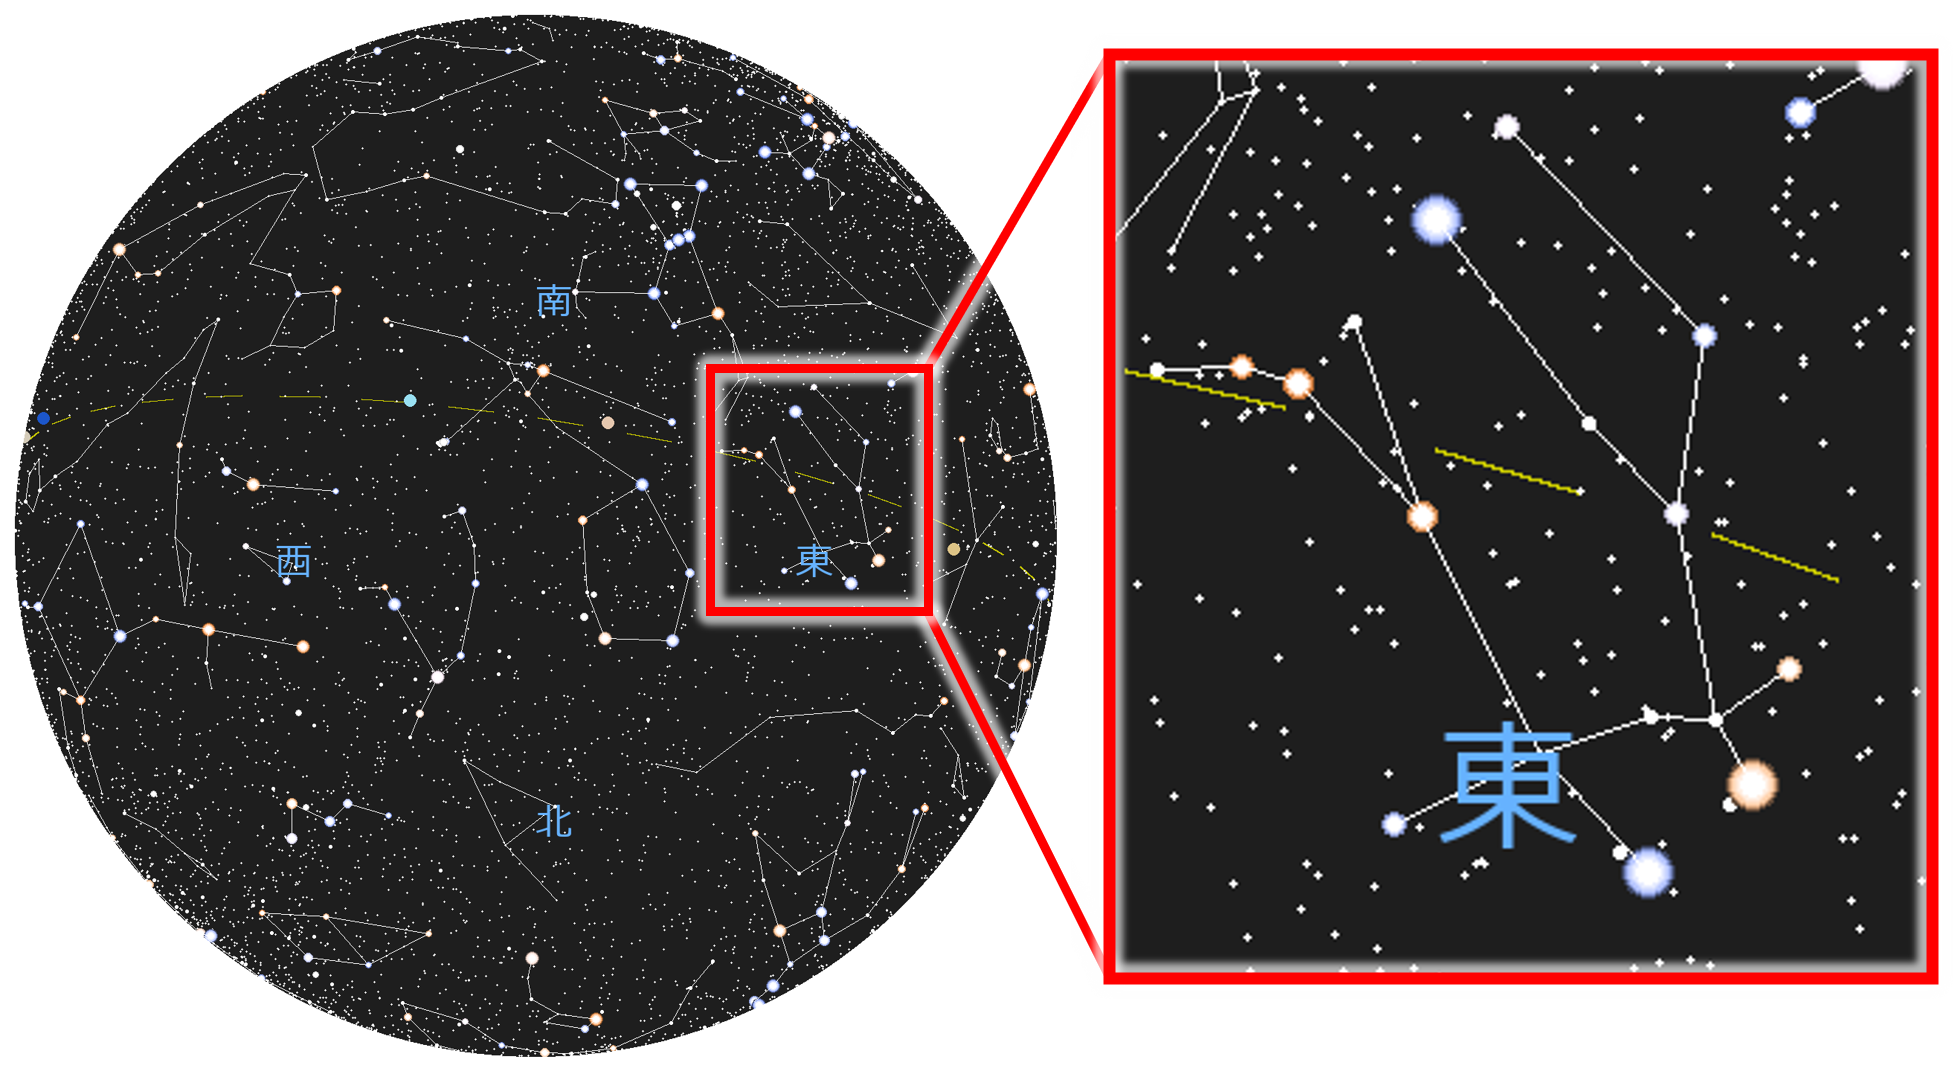
\includegraphics[width=15cm]{sections/Fujisawa/image/planisphere_normal.png}
  \caption{2024年11月25日0時0分0秒の星座早見盤}
  \label{fig01}
\end{figure}
今年の部誌はモノクロ印刷らしいので、紙面版の部誌を読んでいる読者には伝わらないと思うが、星座に含まれる恒星たちはその色までほぼ正確に再現している。さらに、一定以上の明るさの恒星はグラデーションで星の輝きを表現している。図\ref{fig01}の右側の拡大図を見てもらえば、恒星の輪郭周辺がグラデーションになっているのが分かる…かもしれない。

描画した各恒星の位置は「ヒッパルコス星表」を参照している。また、ヒッパルコス星表を含む全てのデータは、Astro Commons$^\text{\cite{bib04}}$というサイトで提供されているcsvファイルをダウンロードして利用した。ちなみに使用したライブラリは、PILやNumpyといった一般的なものだけである(ドヤっ)。


%_______________星座線を球面上に描画する____________________
\section{星座線を球面上に描画する}
注意深い読者は気づいたかもしれないが、図\ref{fig01}を見ると星座線は全て直線で描かれている。これは3D化を行う上であまり好ましくない。球面上に存在する2つの恒星を結ぶ星座線は、球面に張り付いてほしいからである。つまり、星座線は直線ではなく緩やかな曲線(正確には楕円の一部)になっていてほしいのだ。図\ref{fig01}では、2つの恒星の間を直線で結んでいるため、各星座線は球面から若干浮いているように見える。球面に張り付いていない星座線の違和感は、3D化を行うとより一層目立ってくるため、ここは甘えずにしっかりと修正しておく。

さて、球面上に張り付いた星座線をどう描画すればいいだろうか。厳密な曲線を描こうとすると、計算が少々複雑になる。また、大半の星座線はほぼ直線として描画されるため、複雑な計算を行ったところで有意な差が現れるとは思えない。そこで、各星座線をN等分に分割した点の3次元座標を求め、各点を平面上に正射影した点を直線で結ぶことで疑似的な曲線を描くことにした。例えば、ある星座線を4分割する場合は、図\ref{fig:split}のように$\mathbf{a}$と$\mathbf{b}$の間の3点の位置ベクトルを求め、これらをxy平面に正射影した後に直線で順に結んでいくイメージである。正射影は恒星の描画時と全く同じ手順で行うため割愛する。ここでは、2つの恒星の3次元の位置ベクトル$\mathbf{a}$, $\mathbf{b}$が与えられた時、その間を最短距離で結ぶ球面上の線分をN等分に分割する各点の座標を求める。$\mathbf{a}$, $\mathbf{b}$はともに単位ベクトルであり、原点は天球の中心にあるとする。

まず、$\mathbf{a}$, $\mathbf{b}$と同じ平面上に存在し、$\mathbf{a}$に垂直な単位ベクトル$\mathbf{n}$を求める。

図\ref{fig02}のようにベクトル$\mathbf{v}$を定めると、$\mathbf{v}$は次のように書ける。
\begin{eqnarray}
  \mathbf{v} = \mathbf{b} - \cfrac{|\mathbf{b}|\cos{\theta}}{|\mathbf{a}|}\ \mathbf{a}  \label{eq01}
\end{eqnarray}

$\cos{\theta} = \frac{ \mathbf{a} \cdot \mathbf{b} }{ |\mathbf{a}| |\mathbf{b} |}$で表されるので、式\ref{eq01}にこれを代入して整理すると次のようになる。
\[
  \mathbf{v} = \mathbf{b} - \cfrac{\mathbf{a} \cdot \mathbf{b}}{|\mathbf{a}|^2}\  \mathbf{a}
\]
よって、ベクトル$\mathbf{n}$は以下で求まる。
\[
  \mathbf{n} = \cfrac{\mathbf{v}}{|\mathbf{v}|}
\]

\begin{figure}[H]
  \centering
  \begin{minipage}[b]{0.45\linewidth}
    \centering
    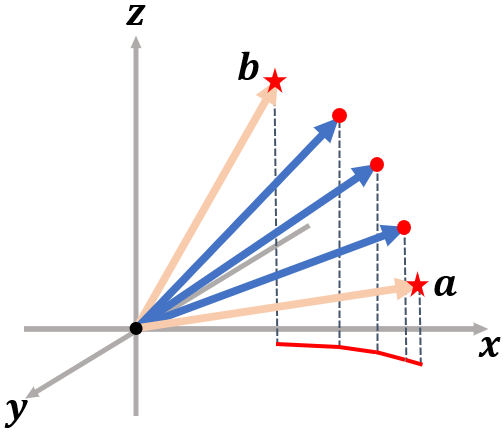
\includegraphics[width=6cm]{sections/Fujisawa/image/starline_split.PNG}
    \caption{星座線を4等分した時の分割点}
    \label{fig:split}
  \end{minipage}
  \begin{minipage}[b]{0.45\linewidth}
    \centering
    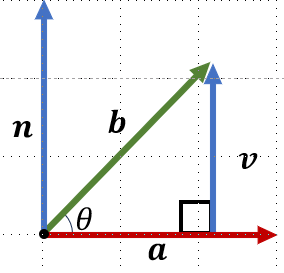
\includegraphics[width=4cm]{sections/Fujisawa/image/n_angle.PNG}
    \caption{単位ベクトル$\mathbf{n}$}
    \label{fig02}
  \end{minipage}
\end{figure}

また、$\theta$は、$\cos$の逆関数を用いて$\theta = \cos^{-1}{\left( \frac{ \mathbf{a} \cdot \mathbf{b} }{ |\mathbf{a}| |\mathbf{b} |} \right)}$で求められる。

$\mathbf{a}$と$\mathbf{b}$を最短距離で結ぶ球面上の線分をN等分した時、$\mathbf{a}$側から数えて$k$番目の点の位置を表すベクトル$\mathbf{x}_k$は、$\mathbf{a}$、$\mathbf{n}$、$\theta$を用いて次のように計算することができる。
\[
  \mathbf{x}_k = \mathbf{a}\cos{\left( \cfrac{k}{N}\ \theta \right)} + \mathbf{n}\sin{\left( \cfrac{k}{N}\ \theta \right)}
\]
これを$k=0$から$k=N$まで計算すれば、各点の3次元座標が求まり、それらを2次元に正射影した後に各点を順番に直線で結んでいけば、目的の星座線を描画することができる。

実際に描画した様子を図\ref{fig03}に示す。直線で描画した星座線(図\ref{fig04})と比較すると曲線になっているのがよく分かる。
\begin{figure}[H]
  \centering
  \begin{minipage}[b]{0.45\linewidth}
    \centering
    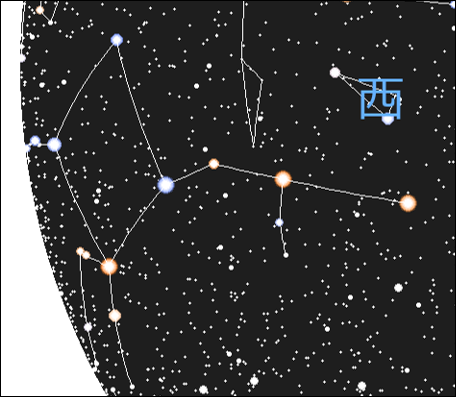
\includegraphics[scale=0.6]{sections/Fujisawa/image/correct_constellations.png}
    \caption{球面上に描画した星座線}
    \label{fig03}
  \end{minipage}
  \begin{minipage}[b]{0.45\linewidth}
    \centering
    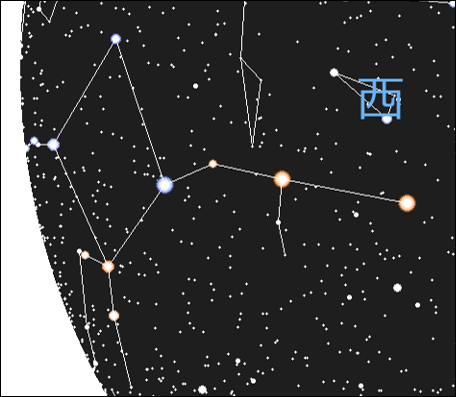
\includegraphics[scale=0.6]{sections/Fujisawa/image/wrong_constellations.png}
    \caption{直線で描画した星座線}
    \label{fig04}
  \end{minipage}
\end{figure}



%________________立体視を用いた3D化_________________
\section{立体視を用いた3D化}
前置きが長くなってしまったが、ここから本記事の主題である「星座早見盤の3D化」について話していく。3D化を行う上で重要になってくるのが立体視である。そもそも立体視が何なのか知らない人のために簡単に説明しておく。人間が何らかの物体を見る時、左右2つの目に映っている像は異なっている(図\ref{fig:stereogram_explain})。この左右の目に映る像の差から、空間上の物体の位置を把握する方法が立体視である。立体視を利用することで、2次元上の画像を立体的に知覚させることができる。方法はシンプルで、同じ物体を2種類の視点から見た画像を用意し、左右の目に別々の画像を見せればよい。

\begin{figure}[H]
  \centering
  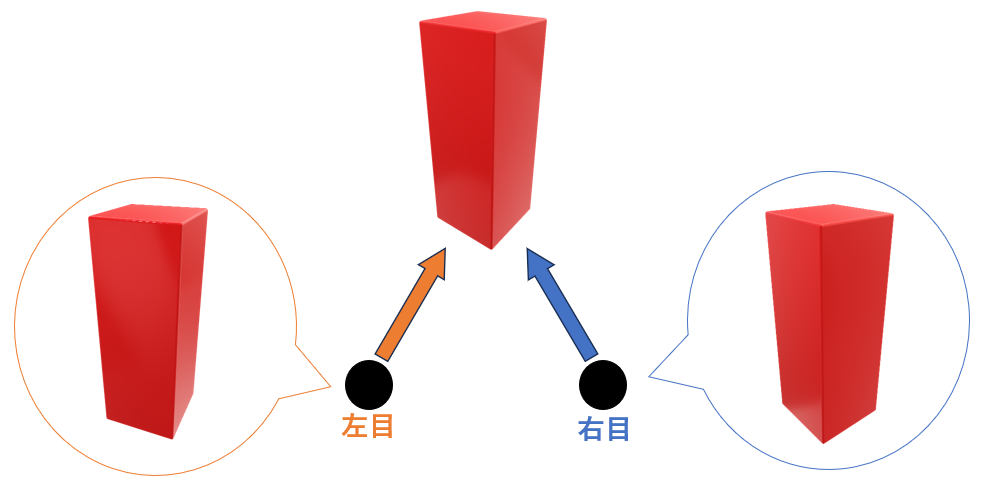
\includegraphics[width=12cm]{sections/Fujisawa/image/stereogram_guidance.PNG}
  \caption{立体視}
  \label{fig:stereogram_explain}
\end{figure}

今回3D化する星座早見盤は、その生成過程で既に各恒星の3次元座標が求まっている。よって、各恒星の3次元座標から立体視によるズレを考慮した射影位置を計算する。図\ref{fig:stereogram_pla_x}は、ある恒星$P(x, y, z)$について、左右の画像におけるx座標の射影位置$x_L$、$x_R$を図示したものである。$Y=y$で切ったXZ平面の様子を表しており、半円は天球の切り口である。また、点$E_L$、$E_R$はそれぞれ左右の目の位置を表している。左目と右目の間の距離は$W$であり、両目とも$XY$平面から距離$H$だけ離れている。また、図\ref{fig:stereogram_pla_y}はy座標の射影位置$y'$を図示したものである。$X=x$で切ったYZ平面であり、両目のy座標は等しいため、左目および右目の位置を$E$で表している。

これまでの射影方法は単なるXY平面への正射影だったので、恒星Pの射影位置は、図\ref{fig:stereogram_pla_x}、図\ref{fig:stereogram_pla_y}それぞれにおける点$x$、$y$であった。
\begin{figure}[H]
  \centering
  \begin{minipage}[b]{0.48\linewidth}
    \centering
    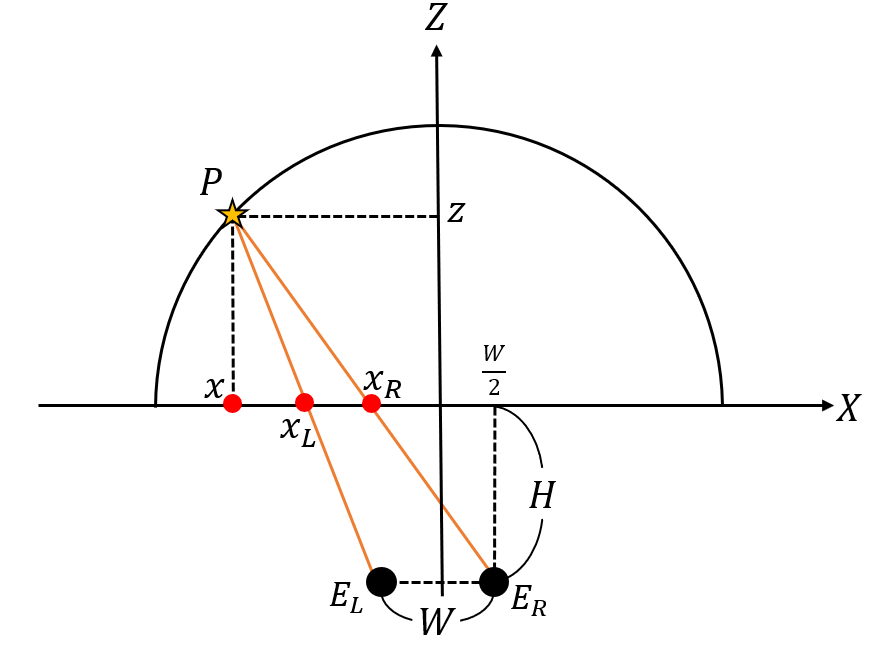
\includegraphics[width=8cm]{sections/Fujisawa/image/stereogram_pla_x.PNG}
    \caption{立体視による射影位置のズレ(x座標)}
    \label{fig:stereogram_pla_x}
  \end{minipage}
  \begin{minipage}[b]{0.48\linewidth}
    \centering
    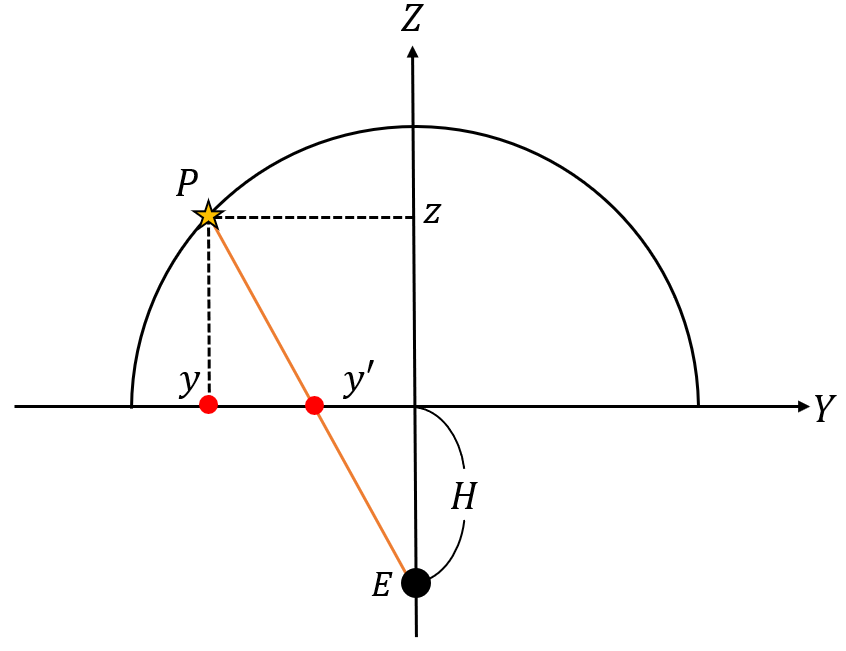
\includegraphics[width=7.5cm]{sections/Fujisawa/image/stereogram_pla_y.PNG}
    \caption{立体視による射影位置のズレ(y座標)}
    \label{fig:stereogram_pla_y}
  \end{minipage}
\end{figure}
立体視によるズレを考慮した場合の射影位置$x_L$、$x_R$、$y'$の座標は図\ref{fig:stereogram_pla_x}、図\ref{fig:stereogram_pla_y}より、それぞれ次の式で計算できる。
\begin{eqnarray*}
  x_L = x - z\left( \cfrac{\frac{W}{2} + x }{z+H} \right)\ \ \ \ \ \ x_R = x + z\left( \cfrac{\frac{W}{2} - x }{z+H} \right) \ \ \ \ \  \ y' = y - z\left( \cfrac{y}{z+H} \right)
\end{eqnarray*}

恒星Pをそれぞれ$(x_L, y')$、$(x_R, y')$に射影した2種類の画像を用意し、左右の目で別々の画像を見れば、星座早見盤を立体的に知覚することができる。

最後に、左右の目それぞれに別々の画像を見せる方法を3つ紹介する。1つ目と2つ目は似ており、それぞれ交差法、平行法と呼ばれている。右目で左の画像を、左目で右の画像を見る方法が交差法であり、逆に右目で右の画像を、左目で左の画像を見る方法が平行法である。3つ目は青赤メガネを使う方法で、アナグリフ方式と呼ばれる。これはちょうど、暗記用の赤い下敷きで赤文字が消えて見えるのと同じ原理を用いている。赤いメガネを通して見ると青色の画像しか見えず、青いメガネを通して見ると赤色の画像しか見えない。これを利用して左右の目に異なる画像を見せることで、立体視が実現できる。図\ref{fig:stereo_glass}は説明用のため、赤い画像と青い画像が実際よりも離れた図になっている。
\begin{figure}[H]
  \centering
  \begin{minipage}[b]{0.32\linewidth}
    \centering
    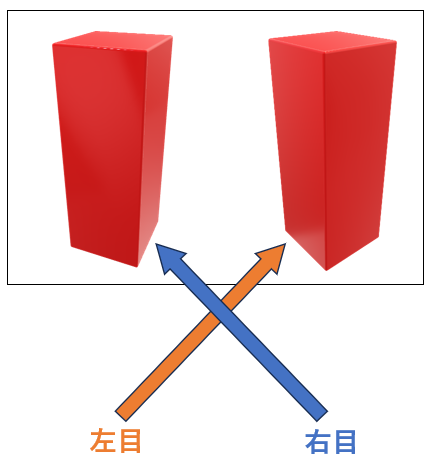
\includegraphics[width=5cm]{sections/Fujisawa/image/stereo_cross.PNG}
    \caption{交差法}
    \label{fig:stereo_cross}
  \end{minipage}
  \begin{minipage}[b]{0.32\linewidth}
    \centering
    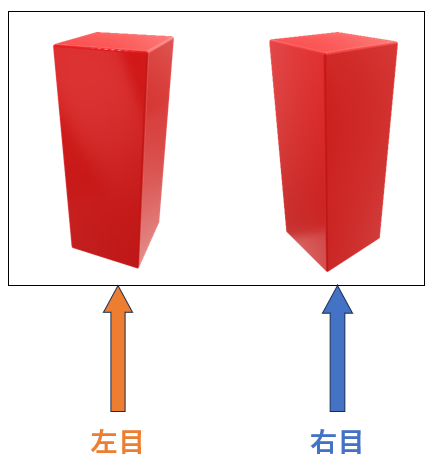
\includegraphics[width=5cm]{sections/Fujisawa/image/stereo_parallel.PNG}
    \caption{平行法}
    \label{fig:stereo_parallel}
  \end{minipage}
  \begin{minipage}[b]{0.32\linewidth}
    \centering
    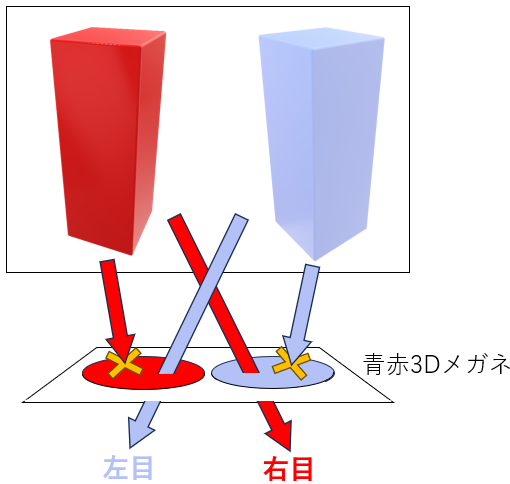
\includegraphics[width=5.7cm]{sections/Fujisawa/image/stereo_glass.PNG}
    \caption{アナグリフ方式}
    \label{fig:stereo_glass}
  \end{minipage}
\end{figure}
次ページに星座早見盤を載せておくので、ぜひ立体視に挑戦してみてほしい(図\ref{fig:stereogram})。モノクロ印刷のため、黒地に白点を描くより白地に黒点を描く方が見やすかったので、恒星と背景の色を反転させている。

\newpage
\begin{figure}[H]
  \centering
  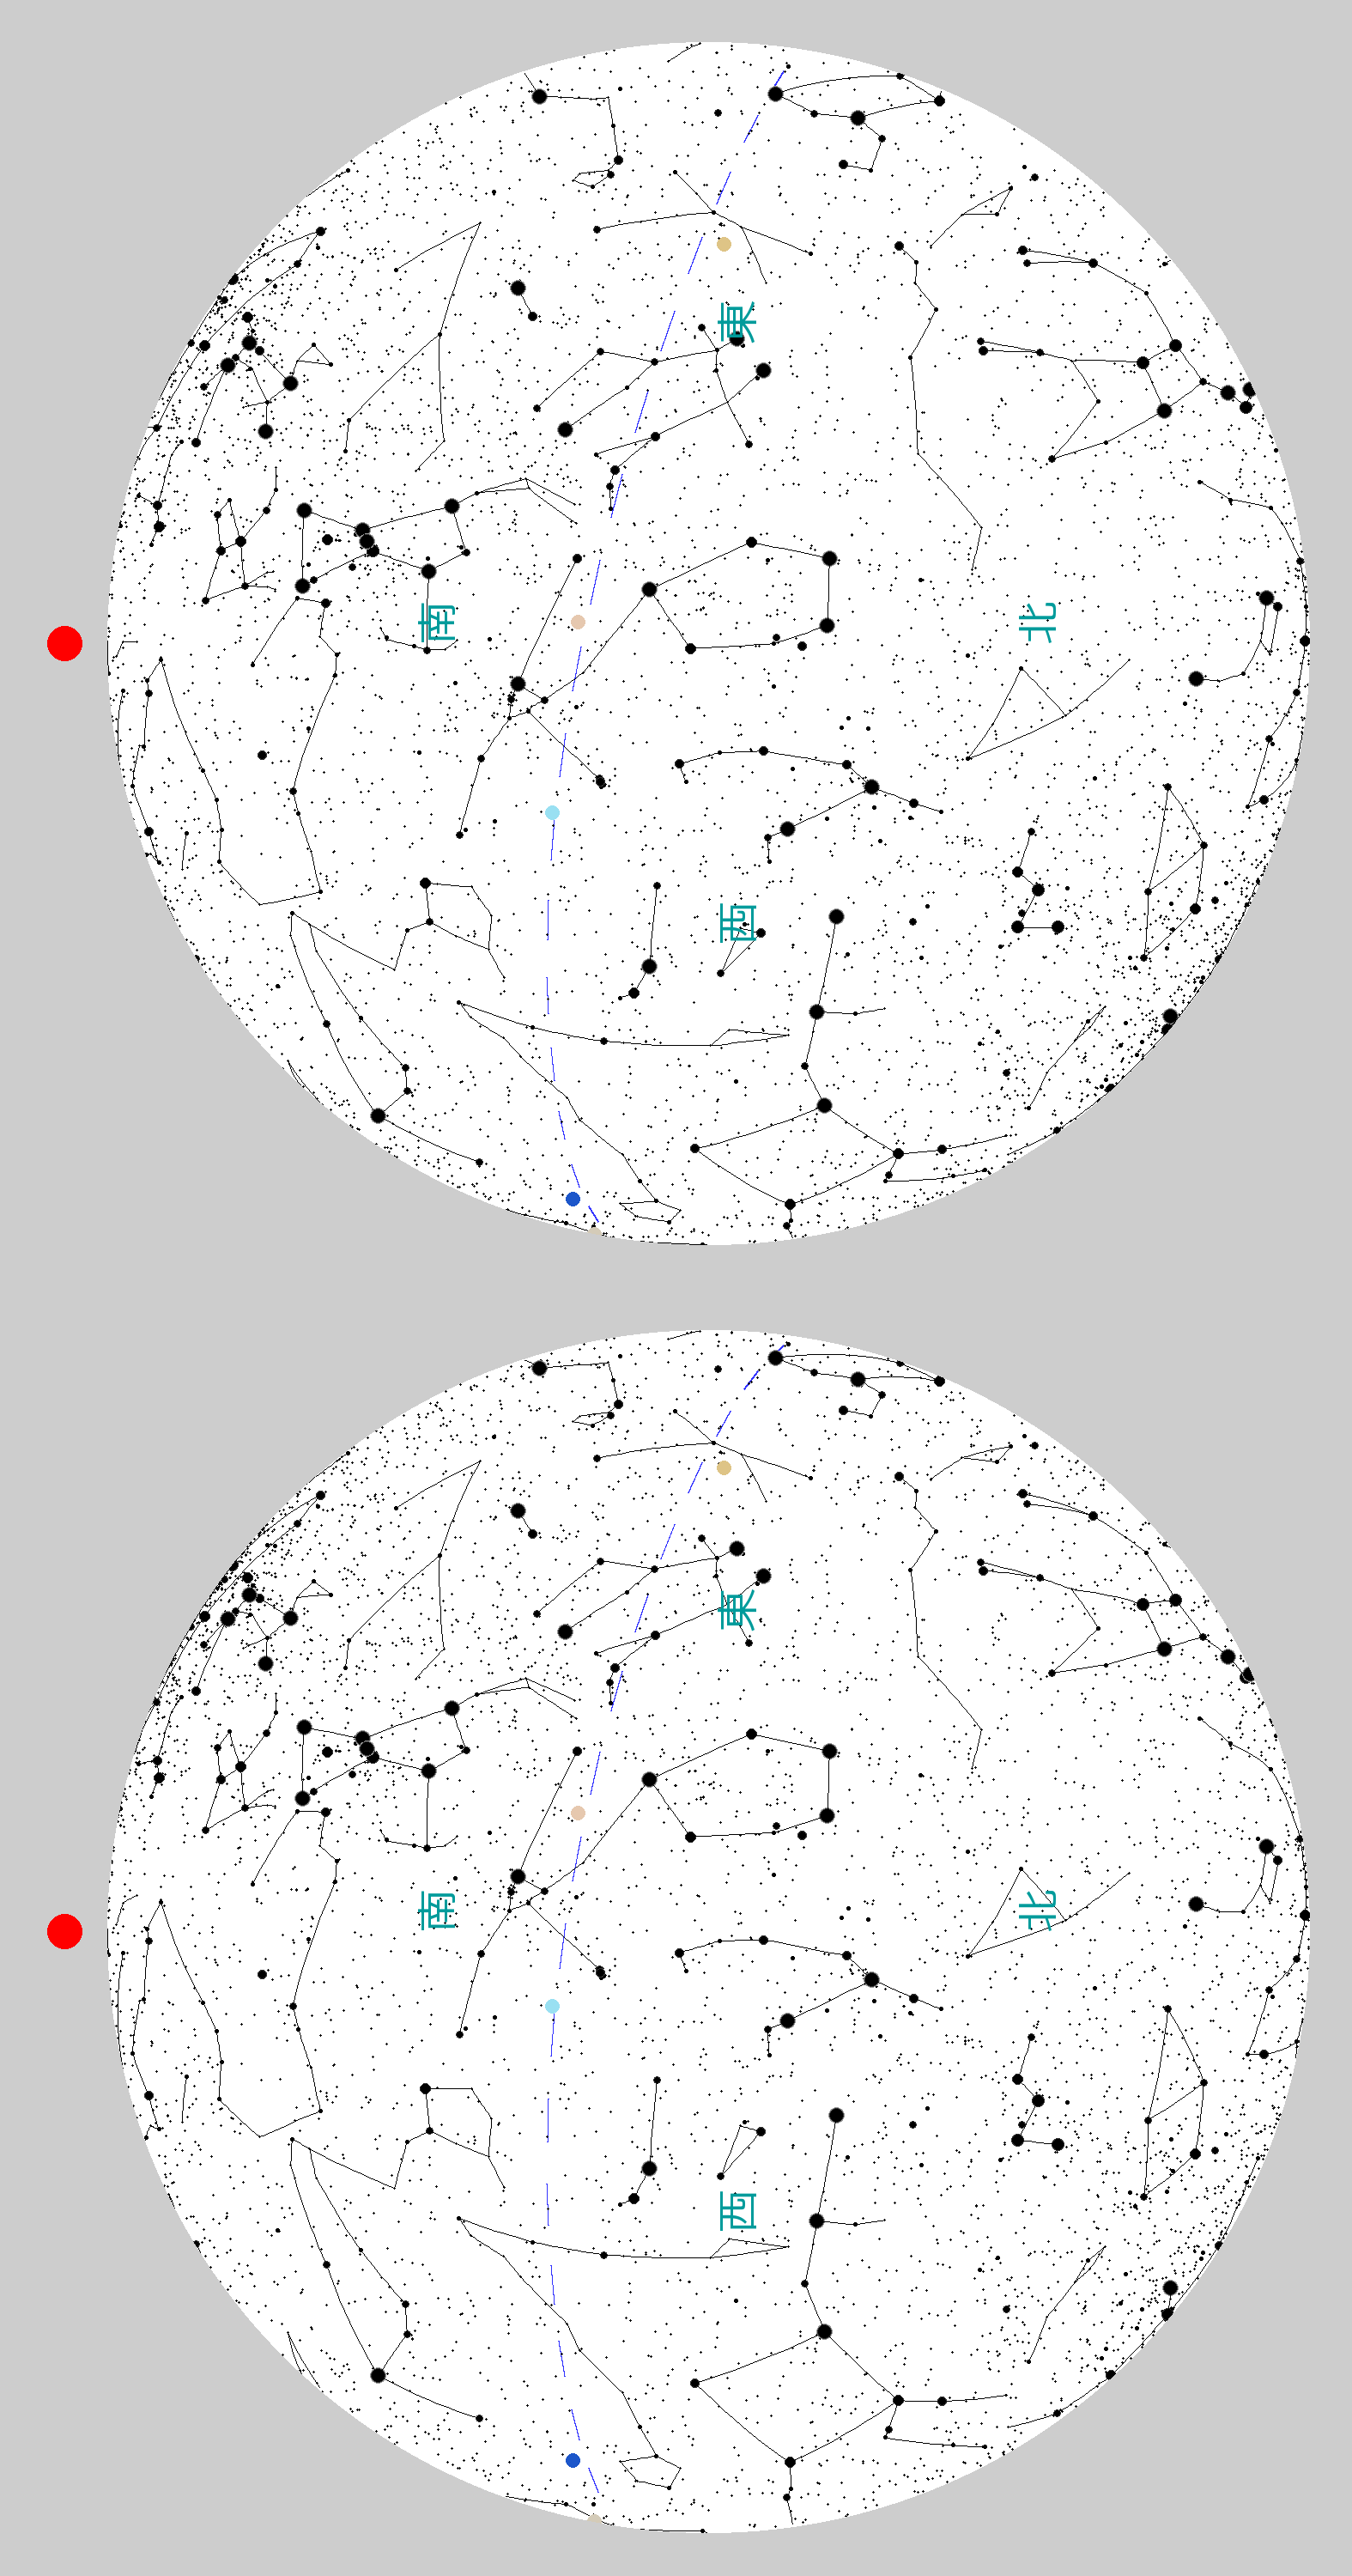
\includegraphics[width=13cm]{sections/Fujisawa/image/CrossEyed_2024_11_25_0_0_0.png}
  \caption{2024年11月25日0時0分0秒の星座早見盤(立体視ver)}
  \label{fig:stereogram}
\end{figure}
\newpage

交差法で描画したため、寄り目で見ると星座早見盤が奥に凹んでいるように見える。また、凹凸は逆になるが、平行法でも立体的に見ることができる。寄り目で見る場合は、まず左右の早見盤の上にある丸い点が重なるように調整する。この時はまだ見ている像がぼやけていても構わない。左の画像、右の画像、そしてその中央に左右を重ねた像が見えている状態にする。この状態のまま、目の力を少し抜きつつピントを合わせれば、半球状に凹んだ星座早見盤が見られるはずである。

立体視ができない人は、寄り目をし過ぎている可能性があるので、もっと目の力を抜いてみるとよい。もしくは、紙と目の距離を離してみると見やすいかもしれない。近くで見すぎると立体視の効果が薄れてしまうため、紙と目は適切な距離を保つ必要がある。

また、交差法や平行法が難しい人向けに、展示教室内に「アナグリフ方式で立体的に見る星座早見盤」が置かれている。青赤メガネを使って、ぜひ3D化された星座早見盤を見ていってほしい。

\begin{thebibliography}{99}
  \bibitem{bib01} 天文部誌「Super Nova」2022調布祭号
  \bibitem{bib02} 天文部誌「Super Nova」2023春号
  \bibitem{bib03} 天文部誌「Super Nova」2023調布祭号
  \bibitem{bib04} Astro Commons (\url{http://astro.starfree.jp/commons/})
\end{thebibliography}

\end{document}
